\section{Conceptos básicos y antecedentes}

En esta sección se va a describir la energía eólica, algunos conceptos básicos de la turbina y tipos de pala. En primera lugar una breve explicación de como surgió la generación de energía mediante los aerogeneradores, después se presentarán las partes básicas de un aerogenerador moderno y por último algunas nociones relacionadas con las palas del aerogenerador y los tipos que existen de este.

\subsection{Energía eólica, historia e ideas básicas}

Actualmente la energía eólica es una de las maneras mas sostenibles para la obtención de energía eléctrica en el mundo. Esta es poco contaminante y pasiva. Se realiza la instalación de la turbina y esta mediante el viento y el giro de sus palas que se traduce en energía mecánica mediante el uso de engranajes que transmiten de manera controlada el movimiento a un generador, produciendo así energía. Esta energía posteriormente es transmitida a centrales eléctricas que la manipulan para que pueda llegar a nuestras casa.\\

En la antigüedad el viento no era utilizado para la obtención de energía tal y como se conoce hoy. Este era aprovechado mediante ciertos sistemas como por ejemplo molinos de viento que se utilizaban para moler grano y obtener harina o por ejemplo sistemas de bombeo de agua para realizar trabajos.\\

No fue hasta el año 1887 que no se construyó lo que se conoce la primera turbina eólica, esta consiguió generar energía eólica y su almacenamiento. Esta era vertical y de gran tamaño.

\begin{figure}[H] 
    \centering
    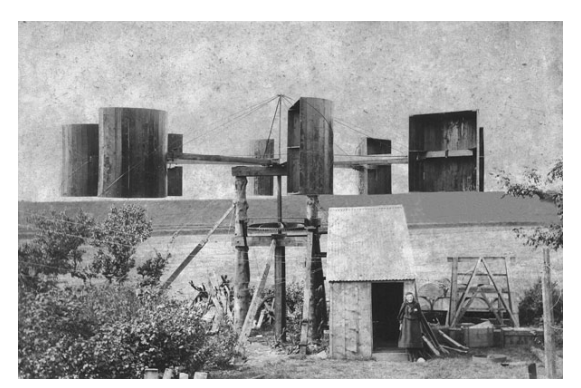
\includegraphics[width=0.8\textwidth]{images/1a turina eolica.PNG}
    \caption{Turbina eólica del Profesor James Blyth con almacenamiento a base de baterías con acumuladores}
    Fuente: Artículo \cite{1aturbina}, Figura 2
    \label{fig:pala_explicar_partes}
\end{figure}

A partir de este punto numerosos países usaron sistemas parecidos, incluso creando granjas de turbinas eólicas. Pero la potencia obtenida por estas era relativamente baja aunque conseguiría competir con los combustibles fósiles.\\

No fue hasta el año 1973 \cite{1973crisis} en el huracán sucesivo de guerras en el medio oeste y el aumento de consumo de combustibles fósiles produjeron  una subida de más de un 200\% en el barril de crudo. Esto llevó al gobierno de los Estados Unidos a impulsar las energía renovables, entre ellas la eólica.\\

Pero el mayor avance se originó en Dinamarca en 1978 \cite{turbinaDanesa}, con la construcción de la Tvindkraft. Esta fue la primera turbina eólica capaz de generar varios Megavatios (MW) de potencia por si sola.\\

En los años posteriores y con motivo del incremento de coste de los combustibles fósiles y la contaminación que estos generan, las energías renovables han mejorado año a año.\\

Actualmente solo se está rozando la punta del iceberg de todo lo que se puede conseguir mediante el uso de estas tecnologías en cuanto a la obtención de energía. Por el momento los estudios más punteros estudian la instalación y mejora de turbinas eólicas marinas.\\




\subsection{La turbina eólica y sus partes}

Existen diversos tipos de rotores según el tipo, los verticales; como el Savonius y los horizontales; como los multipala desarrollados en EEUU y los basados en palas o \textit{HAWT} en inglés. Este último será el usado posteriormente en el trabajo, ya que en la actualidad son los más populares debido a su sencillez y eficiente aprovechamiento de la energía.\\

También se deben conocer las dos principales disposiciones que pueden presentar las turbinas con las que se va a trabajar; \textit{upwind} y \textit{downwind}, también conocidas como \textit{barlovento y sotavento} respectivamente. \\

En este trabajo se usará la disposición \textit{upwind o barlovento}, pero no se girarán las palas usando un ángulo cónico por simplificación.

\begin{figure}[H] 
    \centering
    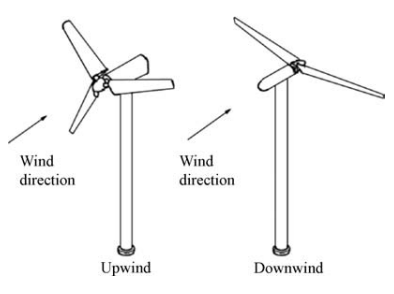
\includegraphics[width=0.6\textwidth]{images/barlovento y sotavento.PNG}
    \caption{Representación por partes básica de una turbina eólica}
    Fuente: Libro \cite{manwell2010wind}, Figura 1.2
    \label{fig:barlovento_sotavento}
\end{figure}

Ahora, se pasa a explicar brevemente cada una de las partes de una turbina eólica completa:

\begin{figure}[H] 
    \centering
    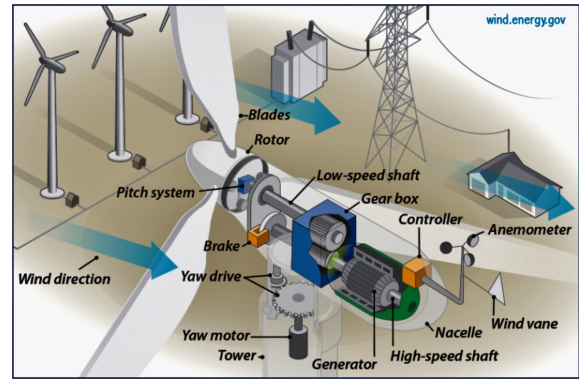
\includegraphics[width=0.9\textwidth]{images/windTurbinebasics.png}
    \caption{Representación por partes básica de una turbina eólica}
    Fuente: Departamento de energía de los Estados Unidos, \cite{usgov}
    \label{fig:pala_explicar_partes}
\end{figure}

\begin{itemize}
  \item Blades o palas: Estructura que causa el giro debido a su forma y posición con respecto al viento.
  \item Pitch system o sistema de cabeceo: Sistema encargado de proporcionar ángulo de cabeceo a las palas.
  \item Rotor: Estructura a la que se encuentran unida las palas y que transmite el giro que realiza al interior de la góndola.
  \item Low-speed shaft o eje de baja velocidad: Eje metálico al que es transmitido el giro del rotor.
  \item Brake o freno: Se encarga de reducir la velocidad de giro de la turbina completa.
  \item Gear box o caja de cambios: Conjunto de engranajes que permiten el aumento de velocidad necesario para el correcto funcionamiento del generador.
  \item Generator o generador: Mecanismo que transforma la energía de rotación o mecánica en energía eléctrica.
  \item High-speed shaft o eje de alta velocidad: Eje conectado al generador que le transmite el giro de la caja de cambios a una alta velocidad.
  \item Controller o controlador: Instrumento electrónico que permite el correcto funcionamiento del sistema generador de energía, como la velocidad de giro de los engranajes, la rotación de la torre o el ángulo de cabeceo de las palas, en parte en base a la información que le transmiten el anemómetro y la veleta.
  \item Nacelle o góndola: Carcasa que contiene todo el sistema eléctrico y mecánico de la turbina eólica.
  \item Anemometer o anemómetro: Dispositivo que realiza mediciones de la velocidad del viento.
  \item Wind vane o veleta de viento: Dispositivo que evalua la dirección del viento.
  \item Yaw drive o unidad de guiñada: Sistema que transmite el giro horizontal de los engranajes de la góndola en verticales de la torre.
  \item Yaw motor o motor de guiñada: Motor que permite a la torre girar para acompañar la dirección del viento.
  \item Tower o torre: Estructura vertical sobre la que se encuentra apoyada la turbina eólica.
  \item Transformador: Aunque no se encuentre en la imagen, supone una parte a destacar ya que aumenta la tensión obtenida una vez ocurrido el proceso de transformación de energía.

\end{itemize}

Algunos conceptos ahora mencionados, son desarrollados más en profundidad a lo largo de este trabajo.

\subsection{Palas de la turbina}

Cientos de trabajos estudian la obtención de una pala óptima, pero generalmente limitada por ciertas condiciones, como pueden ser las atmosféricas o técnicas. Es por ello que es imposible obtener una pala perfecta pero no una óptima para las condiciones con las que se trabajan o bajo las que esté sometida.


\begin{figure}[H] 
    \centering
    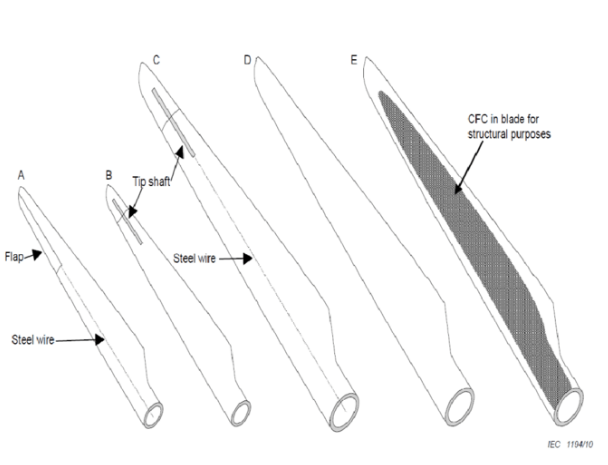
\includegraphics[width=0.8\textwidth]{images/tipos pala.PNG}
    \caption{Representación de algunos de los diferentes tipos de pala de turbina eólica}
    Fuente: Trabajo \cite{Tesauro2014}, Figura 17
    \label{fig:tipos_pala}
\end{figure}

La gran mayoría de turbinas que presentan palas tienen un diseño parecido a las de la figura anterior. Esto se debe a la gran cantidad de estudios realizados alrededor de este elemento. Estos permitieron definir por así denominarlo un estándar en cuanto a la modelización del componente.\\

Una vez se consiguió un diseño estándar se empezó a variar y trabajar con él, produciendo a su vez la investigación acerca de los \textit{airfoils} también conocido como superficies o secciones aerodinámicas. Estas son secciones extraídas de los cortes transversales producidos en la pala. La investigación acerca de estos es crucial en cuanto a la mejora de la construcción de la pala.\\

El diseño y modelización de la pala simplificada con la que se va a trabajar serán definidos en la siguiente sección.